\begin{frame}{Integrated choice and latent variable models}
  \begin{itemize}
    \item Integrated Choice and Latent Variable models are an extension of multinomial logit models
    \item They allow including attitudes in the model specification
    \item The attitudes are included as another \emph{latent variable}, since we don't model them directly
    \item These latent variables are informed by attitudinal indicators
    \item Which indicators go with which latent variables generally based on factor analysis
    \item Also called \emph{hybrid choice models}
  \end{itemize}
\end{frame}

\begin{frame}<1-6>[label=iclv]{Integrated choice and latent variable models}
  \begin{tikzpicture}
    \node[] (force) at (0, 5) {};

    \only<1>{
      \node[draw=black,inner sep=5pt,anchor=west] (ttwalk) at (0, 2) {Travel time by walk};
      \node[draw=black,inner sep=5pt,anchor=west] (ttpt) at (0, 1) {Travel time by transit};
      \node[draw=black,inner sep=5pt,anchor=west] (ttcar) at (0, 0) {Travel time by car};
    }

    \only<2-5,7->{
      \node[draw=black,inner sep=5pt,anchor=west] (tt) at (0, 3) {Travel time};
    }

    \only<1-5,7->{
      \node[draw=black,inner sep=5pt,anchor=west] (inc) at (0, 4) { Income };
      \node[draw=black,inner sep=5pt,anchor=west] (car) at (9, 2) { Probability of car };
      \node[draw=black,inner sep=5pt,anchor=west] (pt) at (9, 3) { Probability of transit };
      \node[draw=black,inner sep=5pt,anchor=west] (walk) at (9, 4) { Probability of walk };

      \node[draw=black,inner sep=5pt,anchor=west,rounded corners=0.2cm] (ucar) at (5, 2) { Utility of car };
      \node[draw=black,inner sep=5pt,anchor=west,rounded corners=0.2cm] (upt) at (5, 3) { Utility of transit };
      \node[draw=black,inner sep=5pt,anchor=west,rounded corners=0.2cm] (uwalk) at (5, 4) { Utility of walk };

      \draw[->] (inc.east) -- ([yshift=3pt]ucar.west) node[pos=0.2,outer sep=0,inner sep=0] (inccar) {};
      \draw[->] (inc.east) -- ([yshift=3pt]upt.west) node[pos=0.25,outer sep=0,inner sep=0] (incpt) {};
      %\draw[->] (inc.east) -- ([yshift=3pt]uwalk.west) node[pos=0.23,outer sep=0,inner sep=0] (incwalk) {};

      % \draw[->] (age.east) -- +(345:2.7cm) -- (ucar.west);
      % \draw[->] (age.east) -- (upt.west);
      % \draw[->] (age.east) -- (uwalk.west);
    }

    \only<1>{
      \draw[->] (ttcar.east) -- ([yshift=-3pt]ucar.west) node[pos=0.2,outer sep=0,inner sep=0] (ttucar) {};
      \draw[->] (ttpt.east) -- ([yshift=-3pt]upt.west) node[pos=0.17,outer sep=0,inner sep=0] (ttupt) {};
      \draw[->] (ttwalk.east) -- ([yshift=-3pt]uwalk.west) node[pos=0.1,outer sep=0,inner sep=0] (ttuwalk) {};
    }

    \only<2-5,7->{
      \draw[->] (tt.east) -- ([yshift=-3pt]ucar.west);
      \draw[->] (tt.east) -- ([yshift=-3pt]upt.west);
      \draw[->] (tt.east) -- ([yshift=-3pt]uwalk.west);

      \draw[->] (ucar.east) -- ([yshift=-3pt]car.west);
      \draw[->] (upt.east) -- (pt.west);
      \draw[->] (uwalk.east) -- ([yshift=3pt]walk.west);

      \draw[->,draw=black!40] (ucar.east) -- ([yshift=-3pt]pt.west);
      \draw[->,draw=black!40] (ucar.east) -- ([yshift=-3pt]walk.west);
      \draw[->,draw=black!40] (upt.east) -- (car.west);
      \draw[->,draw=black!40] (upt.east) -- (walk.west);
      \draw[->,draw=black!40] (uwalk.east) -- ([yshift=3pt]car.west);
      \draw[->,draw=black!40] (uwalk.east) -- ([yshift=3pt]pt.west);

      \draw[<-] (uwalk.north) -- +(90:0.5cm) node[text=black,anchor=south] {$\epsilon$};
      \draw[<-] ([xshift=1em] ucar.south) -- +(270:0.5cm) node[text=black,anchor=north] {$\epsilon$};
      \draw[<-] ([xshift=3em]upt.south) -- +(270:1.5cm) node[text=black,anchor=north] {$\epsilon$};
    }

    \only<3->{
      \node[draw=black,inner sep=5pt,anchor=west,rounded corners=0.2cm] (att) at (3, 0) { Environmental attitude };
    }

    \only<3-5,7->{
      \draw[->] ([xshift=-4em] att.north) -- ([yshift=6pt]uwalk.west);
      \draw[->] ([xshift=-4em] att.north) -- ([yshift=6pt]upt.west);
      \draw[->] ([xshift=-4em]att.north) -- ([yshift=6pt]ucar.west);
    }

    \only<4->{
      \node[draw=black,inner sep=5pt,anchor=west,rounded corners=0.2cm] (globwarm) at (9, 1) { \footnotesize I am concerned about global warming };
      \node[draw=black,inner sep=5pt,anchor=west,rounded corners=0.2cm, text width=5.5cm] (ecology) at (9, 0) { \footnotesize Ecology disadvantages minorities and small businesses };
    }

    \only<5->{
      \draw[->] (att.east) -- (globwarm.west);
      \draw[->] (att.east) -- (ecology.west);
      \draw[<-] ([xshift=2cm]globwarm.north) -- +(90:0.25cm) node[text=black,anchor=south] {$\epsilon$};
      \draw[<-] ([xshift=2cm]ecology.south) -- +(270:0.25cm) node[text=black,anchor=north] {$\epsilon$};
    }

    \only<7->{
      \node[draw=black,inner sep=5pt,anchor=west] (age) at (0, 0) { Age };
      \node[draw=black,inner sep=5pt,anchor=west] (college) at (0, 1) { College educated };
    }

    \only<8->{
      \draw[->] (age.east) -- ([yshift=-3pt]att.west);
      \draw[->] (college.south) -- (att.west);
    }

    \only<9->{
      \draw[<-] (att.south) -- +(270:0.5cm) node[text=black] {$\omega$};
    }
  \end{tikzpicture}
\end{frame}

\begin{frame}{Integrated choice and latent variable models}
  % https://tex.stackexchange.com/questions/44449
  \newcommand*\grayout{black!40}
  \small
  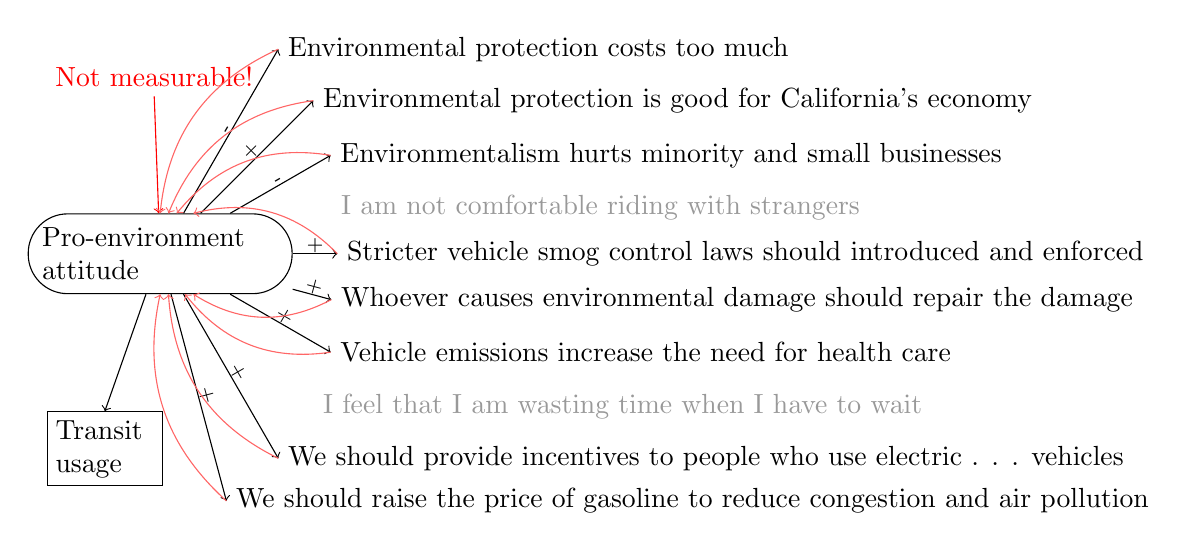
\begin{tikzpicture}
    \node[draw=black,inner sep=5pt,rounded corners=0.5cm,text width=3cm,anchor=east] (attitude) at (3, 5) {\normalsize  Pro-environment attitude};

    \draw[->] ([xshift=-2em]attitude) -- +(270:2cm) node[text=black,anchor=north,text width=1.25cm,inner sep=3pt,draw=black] { Transit usage };


    \draw[<-,color=red] (attitude) -- +([xshift=-0.5ex] 90:2cm) node[text=red,anchor=south] {Not measurable!};


    \node[anchor=west,text=black] (cost) at ([shift=({60:3cm})]attitude) {Environmental protection costs too much};
    \node[anchor=west,text=black] (econ) at ([shift=({45:2.75cm})]attitude) {Environmental protection is good for California’s economy};
    \node[anchor=west,text=black] (hurtssb) at ([shift=({30:2.5cm})]attitude) {Environmentalism hurts minority and small businesses};
    \node[anchor=west,text=\grayout] (strangers) at ([shift=({15:2.25cm})]attitude) {I am not comfortable riding with strangers};
    \node[anchor=west,text=black] (smog) at ([shift=({0:2.25cm})]attitude) {Stricter vehicle smog control laws should  introduced and enforced};
    \node[anchor=west,text=black] (damage) at ([shift=({345:2.25cm)})]attitude) {Whoever causes environmental damage should repair the damage};
    \node[anchor=west,text=black] (emissions) at ([shift=({330:2.5cm})]attitude) {Vehicle emissions increase the need for health care};
    \node[anchor=west,text=\grayout] (time) at ([shift=({315:2.75cm})]attitude) {I feel that I am wasting time when I have to wait};
    \node[anchor=west,text=black] (ev) at ([shift=({300:3cm})]attitude) {We should provide incentives to people who use electric . . . vehicles};
    \node[anchor=west,text=black] (raisegas) at ([shift=({285:3.25cm})]attitude) {We should raise the price of gasoline to reduce congestion and air pollution};

    \draw[->] (attitude) -- (cost.west)
      node[yshift=-0.75ex, midway, above, sloped] {\scriptsize -};
    \draw[->] (attitude) -- (econ.west)
        node[yshift=-0.75ex, midway, above, sloped] {\scriptsize +};
    \draw[->] (attitude) -- (hurtssb.west)
        node[yshift=-0.75ex, midway, above, sloped] {\scriptsize -};
    \draw[->] (attitude) -- (smog.west)
        node[yshift=-0.75ex, midway, above, sloped] {\scriptsize +};
    \draw[->] (attitude) -- (damage.west)
        node[yshift=-0.75ex, midway, above, sloped] {\scriptsize +};
    \draw[->] (attitude) -- (emissions.west)
        node[yshift=-0.75ex, midway, above, sloped] {\scriptsize +};
    \draw[->] (attitude) -- (ev.west)
        node[yshift=-0.75ex, midway, above, sloped] {\scriptsize +};
    \draw[->] (attitude) -- (raisegas.west)
        node[yshift=-0.75ex, midway, above, sloped] {\scriptsize +};


    \path[->,color=red!60,bend right] (cost.west) edge ([xshift=0pt]attitude.north);
    \path[->,color=red!60,bend right] (econ.west) edge ([xshift=3pt]attitude.north);
    \path[->,color=red!60,bend right] (hurtssb.west) edge ([xshift=6pt]attitude.north);
    \path[->,color=red!60,bend right] (smog.west) edge ([xshift=12pt]attitude.north);
    \path[->,color=red!60,bend left] (damage.west) edge ([xshift=12pt]attitude.south);
    \path[->,color=red!60,bend left] (emissions.west) edge ([xshift=9pt]attitude.south);
    \path[->,color=red!60,bend left] (ev.west) edge ([xshift=3pt]attitude.south);
    \path[->,color=red!60,bend left] (raisegas.west) edge ([xshift=0pt]attitude.south);


  \end{tikzpicture}

  {\tiny Based on \textcite{kitamura_micro-analysis_1997}}
\end{frame}
\againframe<5,7->{iclv}

\begin{frame}{Integrated choice and latent variable models: the math}
  \small
  \begin{tabular}{llllll}
    $U_{walk}$ & $=$ &  & $\beta_{time} x_{time,walk}$ & $+ \beta_{walk,environment} \tikzmark{xstar}x*$ & $+ \epsilon_{walk}$ \\
    \\
    $U_{transit}$ & $= \alpha_{transit}$ & $+ \beta_{income,transit} x_{income}$ & $+ \beta_{time} x_{time,transit}$ & $+ \beta_{transit,environment} x*$ &  $+ \epsilon_{transit}$ \\
    \\
    $U_{car}$ & $= \alpha_{car}$ & $+ \beta_{income,car} x_{income}$ & $+ \beta_{time} x_{time,car}$ && $+ \epsilon_{car}$ \\ \\
    \only<2->{
      $x*$ & $= \alpha_{x*} $ & $ + \beta_{x*,age} x_{age}$ & $ + \beta_{x*,college} x_{college}$ & $+ \sigma \tikzmark{omega}\omega$ &
    }\\ \\
    \multicolumn{2}{l}{\only<3->{$I_{global warming}$}} & \only<3->{$= \alpha_{global warming}$ & $+ \beta_{x*,global warming} x*$ & $\epsilon_{global warming}$ &} \\ \\
      \multicolumn{2}{l}{\only<3->{$I_{economy}$}} & \only<3->{ $= \alpha_{economy}$ & $+ \beta_{x*,economy} x*$ & $\epsilon_{economy}$ & }\\ \\
  \end{tabular}

  \begin{tikzpicture}[overlay,remember picture]
    \pause\draw[draw=red,<-] ([xshift=0.5ex,yshift=0.5ex]pic cs:xstar) -- +(90:0.5cm) node[text=red,anchor=south] {Latent attitude};
    \pause\draw[draw=red,<-] ([xshift=0.5ex]pic cs:omega) -- +(325:0.25cm) node[text=red,anchor=north] {Random variable};
  \end{tikzpicture}
\end{frame}

\begin{frame}{Integrated choice and latent variable models: choice model}
  \small
  \centering\begin{tabular}{lrrrr}
    \toprule
    {} &  Value &  Std err &  t-test &  p-value \\
    \midrule
    \hspace*{1em} Travel time (hours)     &  -0.60 &     0.01 &  -61.34 &     0.00 \\
    \hspace*{1em} Walk \\
    \hspace*{1.5em} Environmental attitude&  -0.15 &     0.17 &   -0.89 &     0.37 \\
    \hspace*{1em} Public transit \\
    \hspace*{1.5em} Alternative specific constant &   0.26 &     0.60 &    0.44 &     0.66 \\
    \hspace*{1.5em} Income (tens of thousands of Swiss francs) & -1.42 &     0.10 &  -14.76 &     0.00 \\
    \hspace*{1.5em} Environmental attitude &   0.12 &     0.08 &    1.56 &     0.12 \\
    \hspace*{1em} Car \\
    \hspace*{1.5em} Alternative specific constant &   0.85 &     0.57 &    1.49 &     0.14 \\
    \hspace*{1.5em} Income (tens of thousands of Swiss francs) &  -1.27 &     0.09 &  -13.71 &     0.00 \\
    \bottomrule
  \end{tabular}\\
  \tiny Data: \textcite{bierlaire_mode_2018}
\end{frame}

\begin{frame}{Integrated choice and latent variable models: measurement models}
  \small
  \centering\begin{tabular}{lrrrr}
    \toprule
    {} &  Value &  Std err &  t-test &  p-value \\
    \midrule
    \multicolumn{5}{l}{\textbf{Agreement with ``I am concerned about global warming''}} \\
    \hspace*{1em} Constant & 0\tikzmark{fixed1} & -- & -- & -- \\
    \hspace*{1em} Environmental attitude & 1\tikzmark{fixed2} & -- & -- & -- \\
    \\
    \multicolumn{5}{l}{\textbf{Agreement with ``Ecology disadvantages minorities and small businesses''}} \\
    \hspace*{1em} Constant                &   5.78 &     0.17 &   34.45 &     0.00 \\
    \hspace*{1em} Environmental attitude  &  -0.81\tikzmark{envatt} &     0.05 &  -17.36 &     0.00 \\
  \end{tabular}

  \begin{tikzpicture}[overlay,remember picture]
    \pause\draw[red,<-] ([yshift=0.5ex] pic cs:fixed1) -- +(45:3cm) node[text=red,anchor=west] (fixedcallout) {Fixed};
    \draw[red,<-] ([yshift=0.5ex] pic cs:fixed2) -- (fixedcallout.west);
    \pause\path[red,<->,bend left] (pic cs:fixed2) edge (pic cs:envatt);
  \end{tikzpicture}\\
  \tiny Data: \textcite{bierlaire_mode_2018}
\end{frame}

\begin{frame}{Integrated choice and latent variable models: latent variable model}
  \small
  \centering\begin{tabular}{lrrrr}
    \toprule
    {} &  Value &  Std err &  t-test &  p-value \\
    \midrule
    \hspace*{1em} Constant                &   3.60 &     0.01 &  245.57 &     0.00 \\
    \hspace*{1em} Age (10s of years)      &  -0.02 &     0.00 &   -9.12 &     0.00 \\
    \hspace*{1em} College                 &   0.32 &     0.01 &   27.89 &     0.00 \\
    \hspace*{1em} $\sigma$                &  \tikzmark{sigmazero}$-4\times10^{-6}$ &     0.00 &   -0.01 &     0.99 \\
    \\
  \end{tabular}

  \begin{tikzpicture}[overlay, remember picture]
    \pause\draw[red] ([xshift=2.2em, yshift=0.5ex] pic cs:sigmazero) ellipse (3em and 1.5ex);
    \draw[red,<-] ([xshift=2.2em, yshift=-1ex] pic cs:sigmazero) -- +(270:1cm) node[text=red,anchor=north] {Minimal influence of random variable};
  \end{tikzpicture}\\
  \tiny Data: \textcite{bierlaire_mode_2018}
\end{frame}

\begin{frame}{Integrated choice and latent variable models: real-world example}
  \centering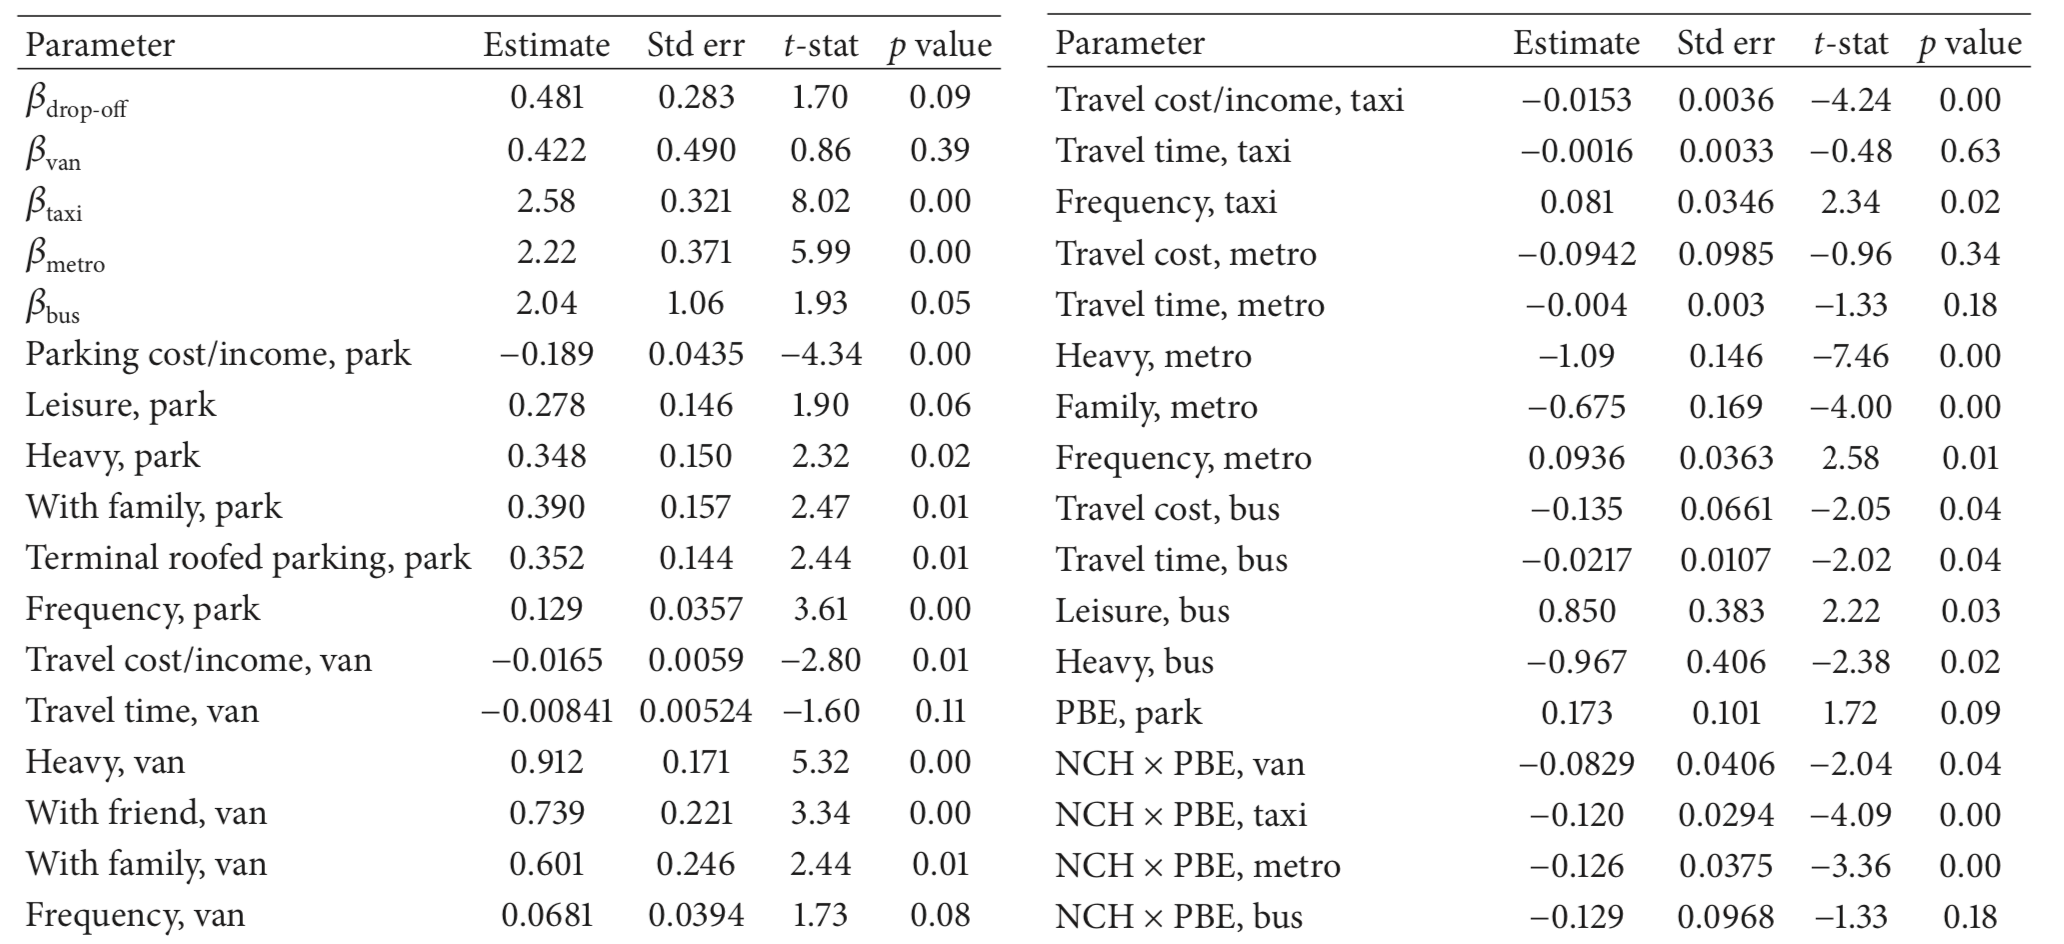
\includegraphics[width=\textwidth]{fig/yazdanpanah_choice.png}\\
  {\tiny \textcite{yazdanpanah_impact_2017}}
\end{frame}

\begin{frame}{Integrated choice and latent variable models: real-world example}
  \centering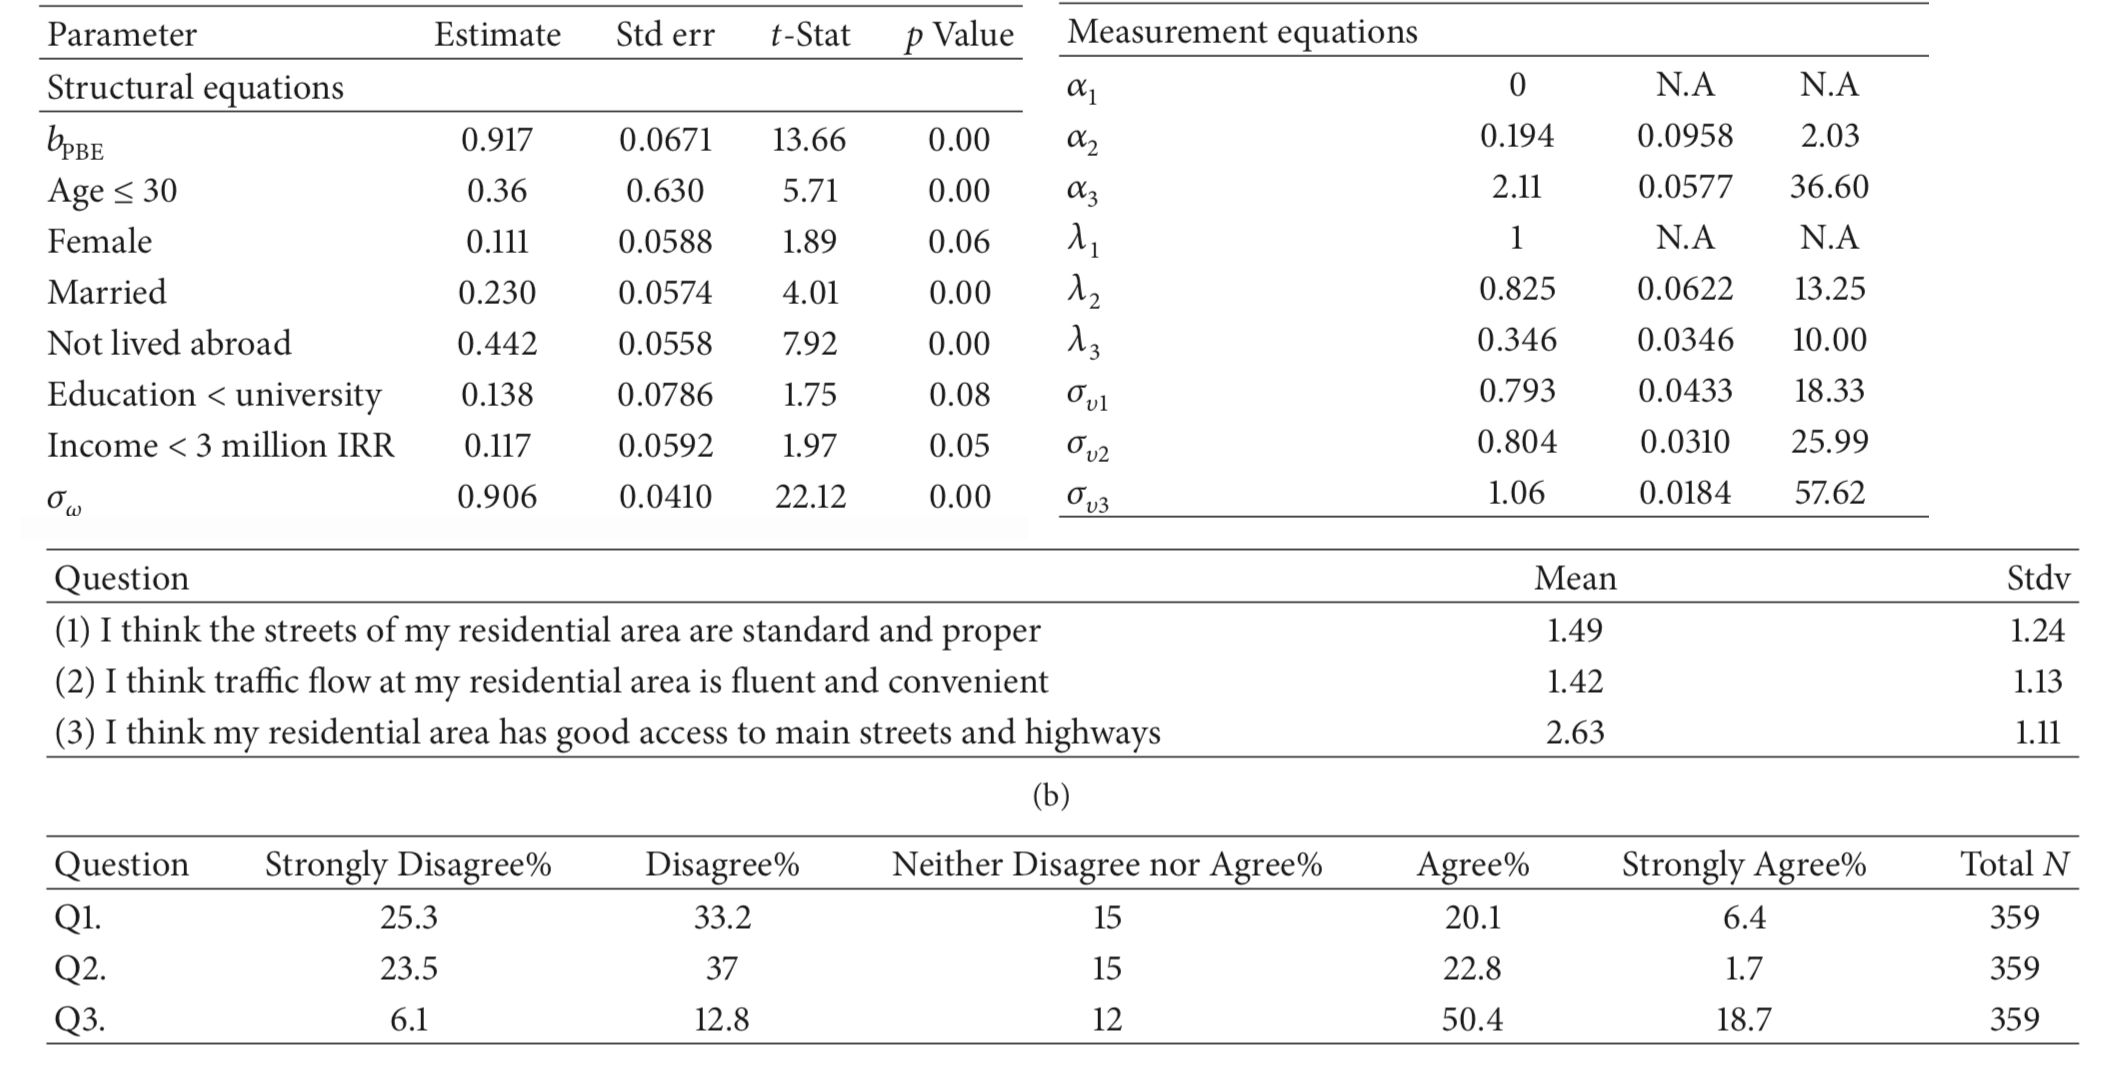
\includegraphics[width=0.8\textwidth]{fig/yazdanpanah_structural.png}\\
  {\tiny \textcite{yazdanpanah_impact_2017}}
\end{frame}

\begin{frame}{Integrated choice and latent variable models: why not just use factor analysis}
  \begin{enumerate}
    \item ICLV models allow finding the combination of indicators that best fits \emph{for this dependent variable}
    \item When doing prediction, the attitudinal indicators do not need to be forecast
  \end{enumerate}
\end{frame}
